Converting the following into a schema:
\begin{figure}[H]
    \centering
    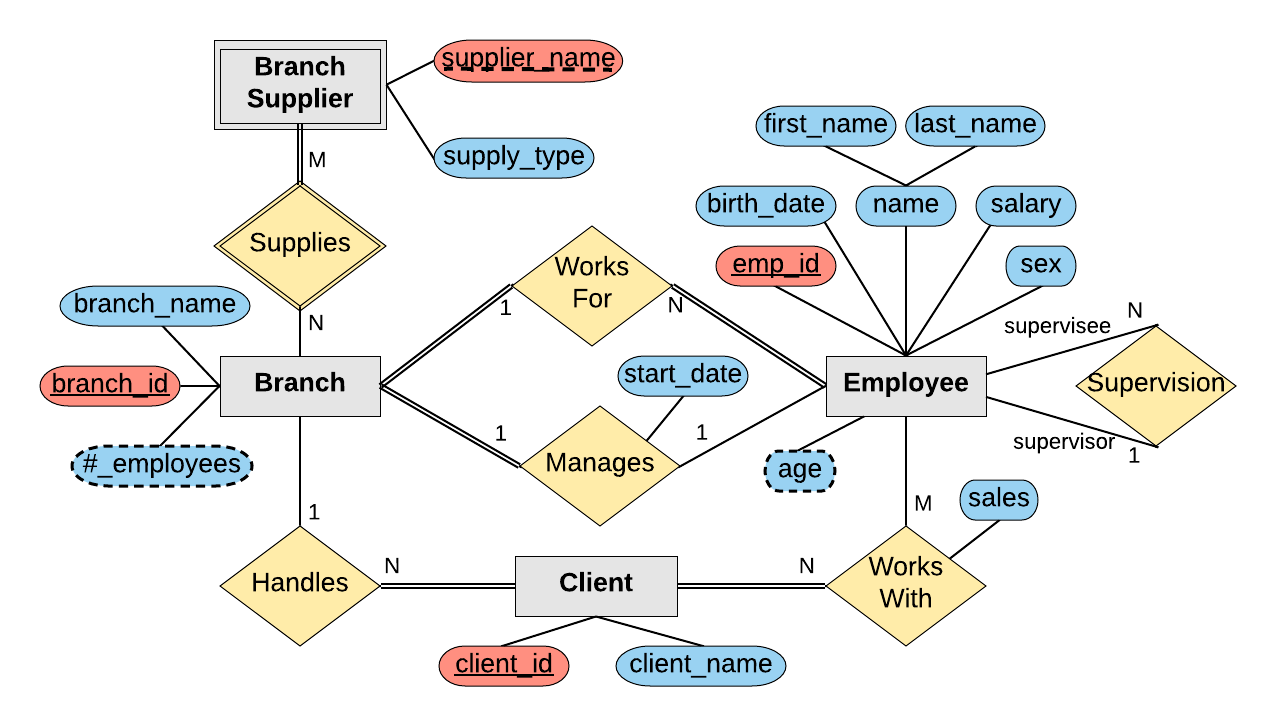
\includegraphics[width=0.8\textwidth]{./Figs/2020-12-24-22-51-10.png}
% 	\caption{}
\end{figure}

\section{Steps}
\begin{enumerate}
    \item Mapping of regular entity types:
        \begin{figure}[H]
            \centering
            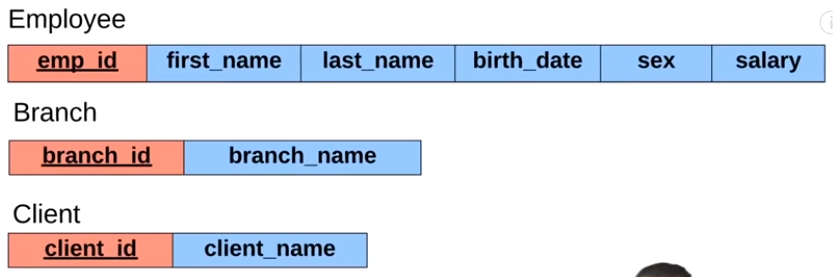
\includegraphics[width=0.4\textwidth]{./Figs/2020-12-24-22-59-55.png}
        % 	\caption{}
        \end{figure}
        \begin{itemize}
            \item For each regular entity type create a relation or table that includes all the simple attributes of that entity.
            \item In this case the regular entities are Branch, Employee, and Client. The columns of the table of the entities will be the simple attributes of the entities.
            \item Notice we don't mark the relationships between the entities nor the branch supplier as an entity because in this case the branch supplier is a weak entity.
            \item In composite attribute it is common to store the attributes that compose the composite attribute rather than storing it as a composite attribute. This means that for example name is composed of first name and last name, but we will not store it as name but rather as first and last name directly. Composite attributes are stored as subattributes.
        \end{itemize}
        \begin{figure}[H]
            \centering
            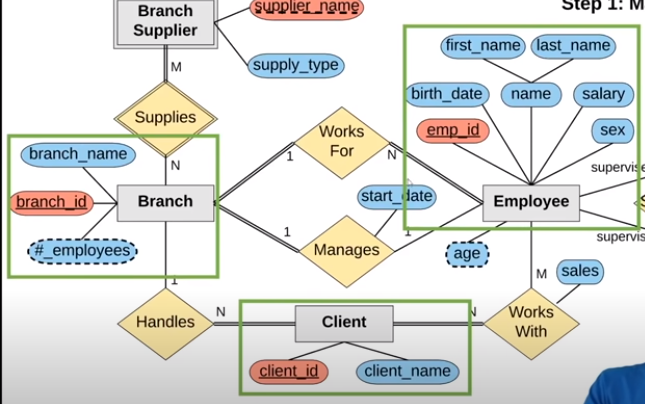
\includegraphics[width=0.4\textwidth]{./Figs/2020-12-24-22-58-24.png}
        % 	\caption{}
        \end{figure}
        
    \item Mapping of weak entity types:
        \begin{figure}[H]
            \centering
            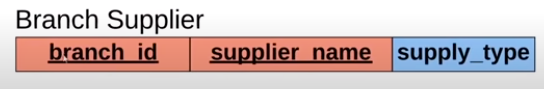
\includegraphics[width=0.4\textwidth]{./Figs/2020-12-24-23-00-07.png}
        % 	\caption{}
        \end{figure}
        \begin{itemize}
            \item For each weak entity type create a relation (table) that includes all simple attributes of the weak entity.
            \item The primary key of the weak entity of the new table should be the partial key of the weak entity plus the primary key of its owner. In this case the primary key will be branch id.
        \end{itemize}
        \begin{figure}[H]
            \centering
            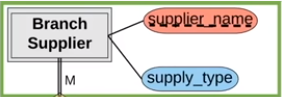
\includegraphics[width=0.4\textwidth]{./Figs/2020-12-24-22-57-54.png}
        % 	\caption{}
        \end{figure}
    
    \item Mapping of Binary 1:1 relationship types:
        \begin{figure}[H]
            \centering
            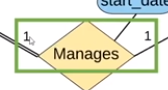
\includegraphics[width=0.4\textwidth]{./Figs/2020-12-24-23-00-49.png}
        % 	\caption{}
        \end{figure}
        \begin{itemize}
            \item For each one to one binary relationship we want to include one side of the relationship as a foreign key in the other favor total participation.
            \item Basically include the primary key of one of these entities as a foreign key in the other's entity relation. And if a particular entity has total participation in the relationship then you want to add the foreign key on to the one that has total participation, in this case to branch, add the employee primary key as a foreign key to branch.
            \item If both of them are total participation or both are partial participation then it is left to your discretion to decide which entity has the foreign key.
            \item To the table Branch, add the foreign key of employee, in this case called mgr\_id will be foreign key to link the relationship.
        \end{itemize}
        \begin{figure}[H]
            \centering
            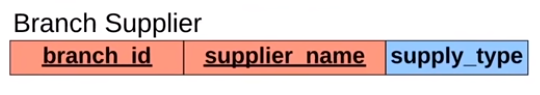
\includegraphics[width=0.4\textwidth]{./Figs/2020-12-24-23-05-49.png}
        % 	\caption{}
        \end{figure}
    
    \item Mapping of binary 1:N relationship types:
        \begin{figure}[H]
            \centering
            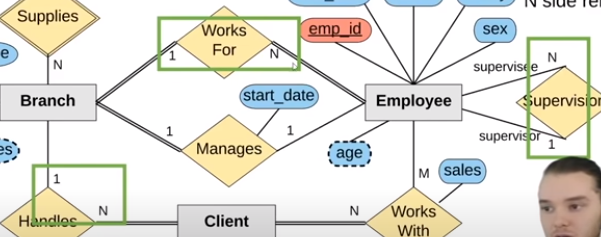
\includegraphics[width=0.4\textwidth]{./Figs/2020-12-24-23-07-54.png}
        % 	\caption{}
        \end{figure}
        \begin{itemize}
            \item Include the 1 side's primary key as a foreign key in the N side relation table.
            \item In this case we have three.
            \item Basically, in the case where we establish the relationship between the branch works for employee, I want to include the 1's side primary key, which means the branch side, as a foreign key in the employee table, this means that employee will have a column as a foreign key specifying the branch.
            \item In the employee supervision relation, we grab the 1's side, which is employee and store in the N's side, which is employee, the foreign key to the supervisor.
            \item In the branch handles client relationship we store as a foreign key a branch in client.
        \end{itemize}
    
    \item Mapping of binary M:N relationship types:
        \begin{figure}[H]
            \centering
            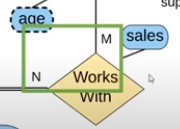
\includegraphics[width=0.4\textwidth]{./Figs/2020-12-24-23-16-49.png}
        % 	\caption{}
        \end{figure}
        \begin{itemize}
            \item Create a new table who's primary key is a combination of both entities' primary key's. Also include any relationship attributes.
            \item In this case store sales.
        \end{itemize}
        \begin{figure}[H]
            \centering
            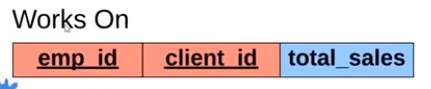
\includegraphics[width=0.4\textwidth]{./Figs/2020-12-24-23-16-39.png}
        % 	\caption{}
        \end{figure}
\end{enumerate}
You should end up with the tables looking like this:
\begin{figure}[H]
    \centering
    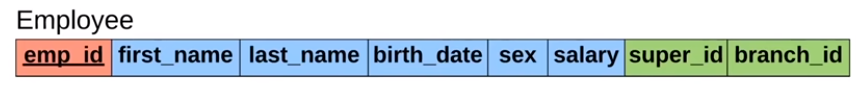
\includegraphics[width=0.4\textwidth]{./Figs/2020-12-24-23-32-40.png}
    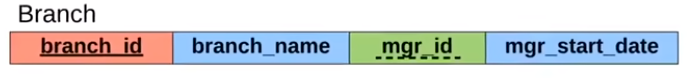
\includegraphics[width=0.4\textwidth]{./Figs/2020-12-24-23-14-01.png}
    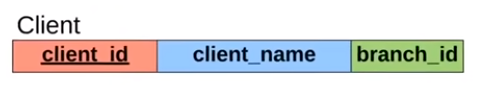
\includegraphics[width=0.4\textwidth]{./Figs/2020-12-24-23-14-09.png}
    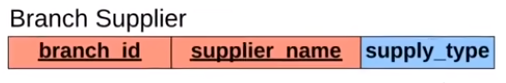
\includegraphics[width=0.4\textwidth]{./Figs/2020-12-24-23-14-17.png}
    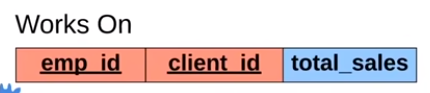
\includegraphics[width=0.4\textwidth]{./Figs/2020-12-24-23-33-07.png}
% 	\caption{}
\end{figure}
You can see the relationships like this:
\begin{figure}[H]
    \centering
    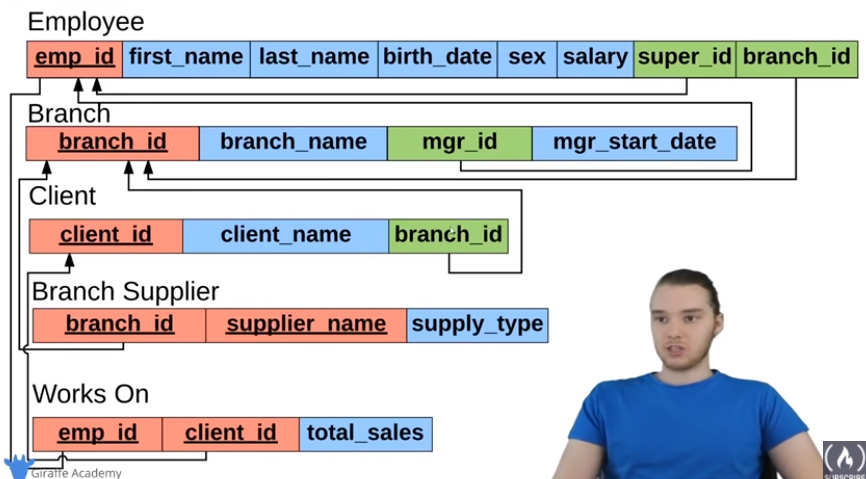
\includegraphics[width=0.4\textwidth]{./Figs/2020-12-24-23-34-55.png}
% 	\caption{}
\end{figure}

Now we can populate the database in the way weve already learned.
\begin{figure}[H]
    \centering
    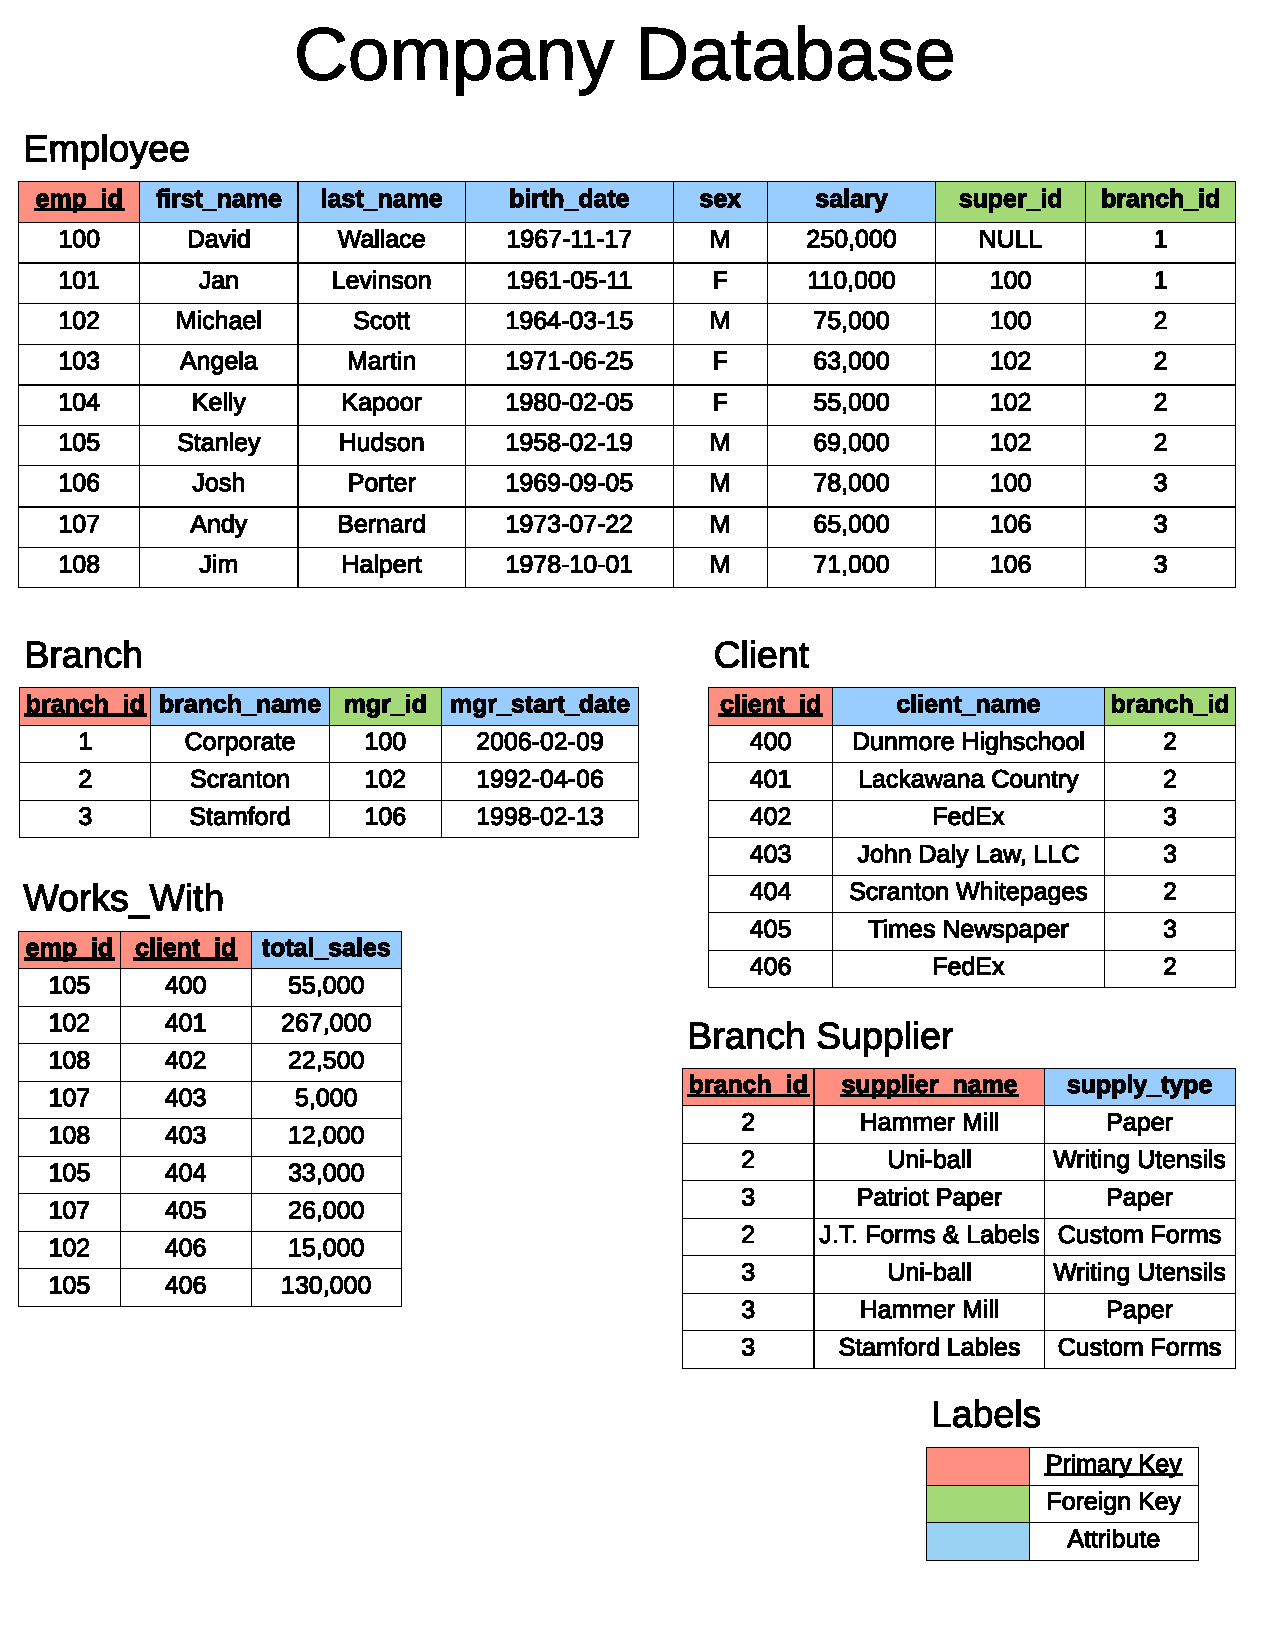
\includegraphics[width=0.8\textwidth]{./Classes/company-database.pdf}
% 	\caption{}
\end{figure}
